\documentclass[a4paper,11pt]{report}

\usepackage[utf8]{inputenx}
\usepackage[style=ieee,citestyle=numeric-comp,backend=biber,alldates=iso8601,maxnames=3]{biblatex}
\usepackage[nottoc]{tocbibind}
\usepackage[font=small,labelfont=bf]{caption}
\usepackage[toc,page]{appendix}
\usepackage{hyperref}
\usepackage{palatino}
\usepackage{newpxmath}
\usepackage{fancyhdr}
\usepackage{lipsum}
\usepackage[margin=3.15cm]{geometry}
\usepackage[toc,nonumberlist,nogroupskip,nopostdot]{glossaries}
\usepackage{graphicx}
\usepackage[english]{babel}
\usepackage{fix-cm}
\usepackage{xcolor}
\usepackage{titlesec}
\usepackage{titlecaps}
\usepackage[abbreviations]{glossaries-extra}
\usepackage[bold]{complexity}
\usepackage[braket, qm]{qcircuit}
\usepackage{tikz}
\usepackage{mathtools}
\usepackage{cleveref}

\usetikzlibrary{arrows.meta}

\pagestyle{fancy}
\cfoot{\thepage}
\lhead[\leftmark]{}
\rhead[]{\leftmark}

\renewcommand*{\arraystretch}{1.1}

\glssetcategoryattribute{general}{glossdesc}{firstuc}
\glssetcategoryattribute{abbreviation}{glossdesc}{title}

\creflabelformat{equation}{#2\textup{#1}#3} % no parentheses when citing equation

\renewcommand{\thefootnote}{\fnsymbol{footnote}}

% Pretty chapter numbering
\definecolor{gray75}{gray}{0.75}
\newcommand{\hsp}{\hspace{0pt}}
\titleformat{\chapter}[hang]{\flushleft
    \fontseries{b}\fontsize{80}{100}\selectfont}{\fontseries{b}\fontsize{100}{130}\selectfont \textcolor{gray75}\thechapter\hsp}{0pt}{\leavevmode\\\Huge\bfseries}[]
\titleformat{name=\chapter,numberless}[hang]{}{}{0pt}{\Huge\bfseries}[]
\titlespacing*{\chapter}{0pt}{0pt}{30pt}

% Variables
\newcommand{\thesistitle}{A High Performance Computing Infrastructure for the Efficient Execution of Hybrid Quantum-Classical Algorithms}
\newcommand{\authorname}{Steven Oud}

\makenoidxglossaries

\newabbreviation{nisq}{NISQ}{noisy intermediate\--scale quantum}
\newabbreviation{hqca}{HQCA}{hybrid quantum\--classical algorithm}
\newabbreviation{hpc}{HPC}{high performance computing}
\newabbreviation{vqe}{VQE}{Variational Quantum Eigensolver}
\newabbreviation{qaoa}{QAOA}{Quantum Approximate Optimization Algorithm}

\addbibresource{graduate-thesis.bib}

\title{\thesistitle}
\author{\authorname\thanks{Tel.: +31621451016}\\
    500776959\\
    \\
    \emph{Faculty of Computer Science, Information Technology,}\\
    \emph{Business IT and Management}\\
    Software Engineering
    \\
    \\
    \\
    Advisor: Marten Teitsma
    \\
    \\
    \\
    Amsterdam University of Applied Sciences\\
    \today}
\date{}

\begin{document}
\begin{titlepage}
\thispagestyle{empty}
    \begin{center}
        \vspace*{1cm}
        \textbf{\LARGE \thesistitle}
        
        \vspace{1.5cm}
        \textit{\large Thesis submitted by}

        \vspace{0.75cm}
        
        \textbf{\large \authorname}
        
        \vspace{0.75cm}
        \textit{\large under the guidance of}
        
        \vspace{0.75cm}
        \textbf{\large Harold Meerwaldt, QuTech\\
            Damian Podareanu, SURF\\
            Richard Versluis, TNO}
        
        \vspace{0.75cm}
        \textit{\large in partial fulfillment of the requirements for the degree of}
        
        \vspace{0.75cm}
        \textbf{\large Bachelor of Science}
        
    \end{center}
\end{titlepage}

\maketitle

\renewcommand{\thefootnote}{\arabic{footnote}}
\pagenumbering{roman}

\chapter*{Abstract}
\lipsum[5]

\cleardoublepage
\tableofcontents

\cleardoublepage
\listoffigures

\cleardoublepage
\listoftables

\cleardoublepage
\pagenumbering{arabic}

\chapter{Introduction}
As an introduction to the work that was done during this thesis, this chapter starts with presenting a brief overview on the relevance of quantum computing, and describing the motivation behind this work.
After that, the objective of this work is described and an outline of this report is given.

\section{Motivation}
Quantum computing is a new model of computation that promises to solve certain problems more efficiently than classical computers by making use of quantum mechanical phenomena such as superposition and interference.
The idea of quantum computing originated from~\textcite{benioff1980computer}, who proposed a quantum mechanical model of the Turing machine in 1980.
This idea was later extended as \textcite{manin1980vychislimoe} and \textcite{feynman1982simulating} independently suggested that quantum computers have the potential to solve certain computational problems intractable by classical computers.
Since then, researchers have been searching for applications for quantum computing.
Some noteworthy developments in the field of quantum computing include Shor's algorithm for factoring integers~\cite{shor1999polynomial} and Grover's algorithm for unstructured database search~\cite{grover1996fast}.
These quantum algorithms promise an exponential and quadratic speedup respectively over their best-known classical counterparts.
The finding of such speedups have catalyzed research towards quantum computers, and more applications have since been found in fields including chemistry~\cite{mcardle2018quantum}, cryptography~\cite{bennett2014quantum}, and machine learning~\cite{biamonte2017quantum}.

Until recently, quantum computing had been a mainly theoretical field.
These days, however, thanks to recent technological advances, various quantum devices are being actively developed.
Furthermore, technological giants such as IBM, Microsoft, Intel, and Google are investing heavily in the development of quantum computers.
The applications of these current quantum devices are very limited however, due to their inability to store information for a long time and their sensitivity to errors.
For instance, \textcite[Appendix~M]{fowler2012surface} estimate that to factor a 2000-bit number using Shor's algorithm would require a quantum computer with about a billion physical qubits, and error rates below $4 \times 10^{-13}$.
In contrast, devices today have about 50 to 100 physical qubits with error rates above $0.1$.

These small and error-prone quantum devices, referred to as \gls{nisq} devices, may be unfit to run quantum algorithms like Shor's algorithm, but they may still prove to be useful and perform tasks intractable by classical computers~\cite{preskill2018quantum}.
To deal with the limitations of \gls{nisq} devices, \glspl{hqca} are being actively researched.
These \glspl{hqca} combine classical and quantum computations as visualized in~\Cref{fig:hybrid-quantum-classical}.
\begin{figure}[ht]
    \centering
    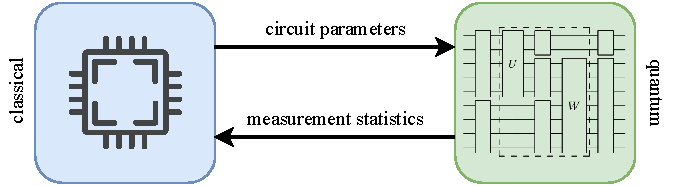
\includegraphics[width=0.65\linewidth]{figures/hybrid-quantum-algorithm.pdf}
    \caption[General structure of a hybrid quantum-classical algorithm.]{General structure of a hybrid quantum-classical algorithm. The data interchange between the classical and quantum part is often repeated many times.}
    \label{fig:hybrid-quantum-classical}
\end{figure}
\Acrlongpl{hqca} typically involve a small quantum computation inside of a classical optimization loop, greatly reducing the amount of quantum resources needed.
This makes them suitable to run on \gls{nisq} devices, and are expected to be one of the first useful applications for quantum computing~\cite{endo2021hybrid}.
It is important to note that \gls{nisq} devices running \glspl{hqca} will likely not be revolutionary by itself.
Instead, it should be seen as an important stepping stone towards more powerful quantum devices and algorithms.

Research towards \glspl{hqca} often involves executing quantum circuits on actual quantum chips or through quantum circuit simulation.
To support this kind of research, classical and quantum computing facilities are needed.
Furthermore, these facilities need to be connected and able to interchange data in a timely manner for this kind of research to be feasible.
This is especially challenging given that both quantum and classical resources are shared with other users.


\section{Objective}
The purpose of this thesis is to propose an infrastructure for the efficient execution of \acrlongpl{hqca}.
This work is in collaboration with TNO, QuTech, and SURF, and is focused on the efficient execution of \glspl{hqca} using QuTech's quantum computing platform Quantum Inspire~\cite{last2020quantum} and SURF's \gls{hpc} center.
To allow for the efficient execution of \glspl{hqca}, the SURF \gls{hpc} and Quantum Inspire job schedulers should be synchronized to minimize the execution of the algorithm.
A key part in this is figuring out sources of overhead and current bottlenecks.
In a hybrid setup like this, overheads such as quantum and classic scheduling wait times, data transfers, and resource initialization can quickly increase the run time of \glspl{hqca}.

%Currently, there are four ways to run quantum computations using Quantum Inspire: running the QX quantum computer simulator on local resources, using Quantum Inspire's QX-26 simulator running on their commodity server, using the QX-31 simulator running on SURF's infrastructure, or using QuTech's Spin-2 or Starmon-5 \gls{qpu}.


\section{Outline}
This report is structured as follows. \Cref{chap:background} provides the reader with a background on computational complexity, quantum information, and quantum computation. \Cref{chap:hybrid-quantum-classical-algorithms} takes a deeper look into well-known \glspl{hqca} and their working.
\Cref{chap:practical-hybrid-quantum-classical-computing} demonstrates the practical execution of \glspl{hqca} using Quantum Inspire and SURF's \gls{hpc} center.


\chapter{Background} \label{chap:background}
This chapter is focused on making the reader familiar with concepts used throughout this report.
First, an introduction to computational complexity is given to establish a mathematical framework to describe the efficiency of computer algorithms.
Second, the basic ideas of quantum information theory are presented.
Finally, an overview of quantum computation is given.

\section{Computational Complexity}
In computer science, there seems to be a fundamental limit to what problems we can solve.
Some problems seem to be inherently uncomputable: there exists no general solution that does not go into an infinite loop for certain inputs~\cite{church1936note, turing1937computable}.
This report will not go further into what problems are computable and uncomputable.
Rather, it will look at the computational efficiency of certain algorithms: how much resources are required to solve a problem?

\subsection{Big-O Notation}
The time and space taken by an algorithm generally grows as the size of the input grows.
Because of this, it is traditional to describing the efficiency of an algorithm as a function of the size of its input~\cite{cormen2009introduction}.
This function describes the number of primitive operations it performs for a given input size.
The notion for input size here depends on the context of the problem.
For example, when computing the discrete Fourier transform, the input size refers to the dimension of the input vector.
When talking about a problem like integer multiplication however, it is more fitting to talk about the input size as the amount of bits needed to represent the input in binary.

When analyzing the efficiency of algorithms, we look at the asymptotic growth for given input size.
Consider an algorithm that given input size $n$ takes $n^2$ primitive operations to run, and another algorithm that takes $500n^2 + \log n$ primitive operations to run.
In big-O notation, both these algorithms are said to run in $O(n^2)$ (quadratic) time.
That is, the amount of primitive operations it performs scales quadratically with the input size.
Constant factors are ignored as they become negligible as $n \to \infty$.
While they are practically significant --- an algorithm which runs in $O(n/2)$ runs twice as fast as an algorithm which runs in $O(n)$ --- they are not relevant to asymptotic analysis. 

Formally, if we have functions $f(n)$ and $g(n)$ such that $f$ eventually grows slower than some multiple of $g$ as $n \to \infty$, we say $f(n) = O(g(n))$.
For example, given $f(n) = 200n^2$ and $g(n) = n^3$, $f$ begins to grow slower than $g$ when $n > 200$.
Thus, $g$ bounds $f$ from above, and $f(n) = O(g(n)) = O(n^3)$.
Some common big-O run times are shown in \Cref{table:common-big-o}, along with their written name and an example.
Throughout this report, algorithms that are bounded above by a polynomial (i.e. all run times until polynomial in \Cref{table:common-big-o}) will be referred to as polynomial-time algorithms, and algorithms that are not bounded above by a polynomial will be referred to as superpolynomial-time algorithms.

\begin{table}[ht]
    \centering
    {\renewcommand{\arraystretch}{1.1}
    \begin{tabular}{ c|c|c }
        Notation & Name & Example \\
        \hline
        $O(1)$ & Constant & Accessing single element from array \\
        $O(\log n)$ & Logarithmic & Binary search \\
        $O(n)$ & Linear & Unstructured database search \\
        $O(n \log n)$ & Linearithmic & Fast Fourier Transform \\
        $O(n^2)$ & Quadratic & Insertion sort \\
        $O(n^k)$ & Polynomial & Gaussian elimination \\
        $O(k^n)$ & Exponential & Graph coloring \\
        $O(n!)$ & Factorial & Brute-force search traveling salesman problem \\
    \end{tabular}
    }
    \caption{Common big-O run times from fast to slow.}
    \label{table:common-big-o}
\end{table}

\subsection{Turing Machines}
The previous section described the measurement of computational efficiency as the number of primitive operations it performs for a given input size.
This abstract definition can be extended by choosing a computational model in order to define what a primitive operation means.
The standard computational model used for this is the Turing machine.
It is chosen as computational model for the analysis of computational efficiency because of its simplicity and because it is able to simulate most physically realizable computational models with little overhead~\cite{arora2009computational}.
An exception to this is the quantum computational model: as far as we know, no classical Turing machine can efficiently simulate a quantum computer~\cite{deutsch1985quantum}.

%A Turing machine is an abstract machine that manipulates symbols on one or multiple infinite length tapes divided into cells~\cite{turing1937computable}.
%Formally, a Turing machine $M$ can be describes by a tuple $(\Gamma, Q, \delta)$ containing:

\subsection{Complexity Classes}
Complexity classes are sets of computational problems that share some common feature with regard to the computational resources they need to solve some problem~\cite{arora2009computational}.
They are defined in terms of a type of computational problem, computational model, and a bounded resource such as time or space.
In general, most complexity classes describe decision problems solvable by deterministic Turing machines --- though many complexity classes are defined in terms of other types of problems and computational models.
This report mainly focuses on complexity classes involving Turing machines and quantum Turing machines.

The class $\P$ contains all decision problems solvable by a deterministic Turing machine in $O(n^k)$ (polynomial) time for some constant $k$.
Problems that fall under this class are often referred to as tractable or easy problems~\cite{cormen2009introduction}.

\section{Quantum Information}

\section{Quantum Computation}

\chapter[Hybrid Quantum-Classical Algorithms]{Hybrid Quantum-Classical\\Algorithms} \label{chap:hybrid-quantum-classical-algorithms}

\section{Variational Quantum Eigensolver}

\section{Quantum Approximate Optimization Algorithm}

\chapter[Practical Hybrid Quantum-Classical Computing]{Practical Hybrid Quantum-Classical\\Computing} \label{chap:practical-hybrid-quantum-classical-computing}
This chapter is focused on the practical execution of \glspl{hqca} using the Quantum Inspire quantum computing platform and SURF's \gls{hpc} center.
First, an overview of the classical and quantum infrastructure is given.
Then, \glspl{hqca} discussed in \Cref{chap:hybrid-quantum-classical-algorithms} are implemented and used for benchmarking and identifying the bottlenecks of the current infrastructure.

\section{Quantum Inspire and SURF Infrastructure}
%Currently, there are four ways to run quantum computations using Quantum Inspire: running the QX quantum computer simulator on local resources, using Quantum Inspire's QX-26 simulator running on their commodity server, using the QX-31 simulator running on SURF's infrastructure, or using QuTech's Spin-2 or Starmon-5 \gls{qpu}.

\section{Implementation}

\section{Benchmarks}

\chapter{Conclusion}

\cleardoublepage
\printbibliography[heading=bibintoc]

\cleardoublepage
\printnoidxglossaries

\end{document}